%! TEX program = xelatex
\documentclass[10pt]{beamer}


\usetheme[progressbar=frametitle]{metropolis}
\setsansfont[BoldFont={Fira Sans}]{Fira Sans Light}
\setmonofont{Fira Mono}
\usepackage{appendixnumberbeamer}

\usepackage{booktabs}
\usepackage[scale=2]{ccicons}

\usepackage{pgfplots}
\usepgfplotslibrary{dateplot}

\usepackage{xspace}
\newcommand{\themename}{\textbf{\textsc{metropolis}}\xspace}

\title{Tecniche di animazione 3D nella realizzazione di un cortometraggio}
\subtitle{}
% \date{\today}
\date{10 Dicembre 2019}
\author{Leonardo Marini}
\institute{ALMA MATER STUDIORUM - UNIVERSITÀ DI BOLOGNA}
%\titlegraphic{\hfill
\includegraphics[height=1.5cm]{logo.pdf}}

\begin{document}

\maketitle

\begin{frame}{Indice}
  \setbeamertemplate{section in toc}[sections numbered]
  \tableofcontents%[hideallsubsections]
\end{frame}

\section[Intro]{Introduzione}

\begin{frame}{Analisi} 
      \begin{itemize}[<+- | alert@+>]								% L'obiettivo della mia tesi è quello di realizzare un 
        \item Cortometraggio animato in 3D 					% cortometraggio con l'uso della computer grafica e, nella sua progettazione,
        \item Uso di diverse tecniche di animazione % analizzare le tecniche di animazione 3D che vengono solitamente usate.
        \item Breve durata 													% Dati i vincoli sulla durata di massimo 2 minuti si è scelto di realizzare solo il trailer.
				\item Nessun requisito sulla storia 				% Non sono stati dati altri vincoli, per quanto riguarda la storia
      \end{itemize}
\end{frame}

\begin{frame}[fragile]{La storia} % Per quest'ultima si è scelto di rappresentarne una ideata dal mio collega... spiegazione
  \begin{columns}[T,onlytextwidth]
    \column{0.33\textwidth}
      \begin{figure}
          \centering
          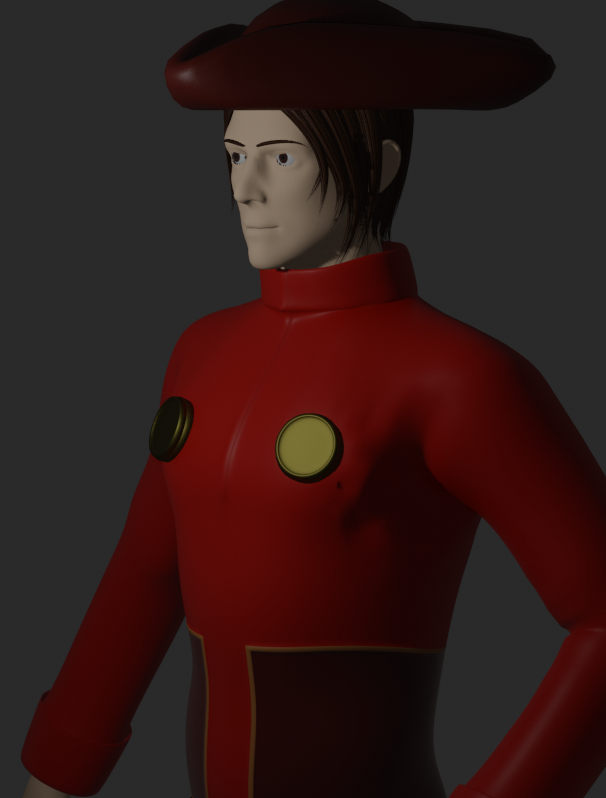
\includegraphics[width=\textwidth]{figures/Capitano.png}
          \caption{Capitano}
      \end{figure}

    \column{0.33\textwidth}
      \begin{figure}
          \centering
          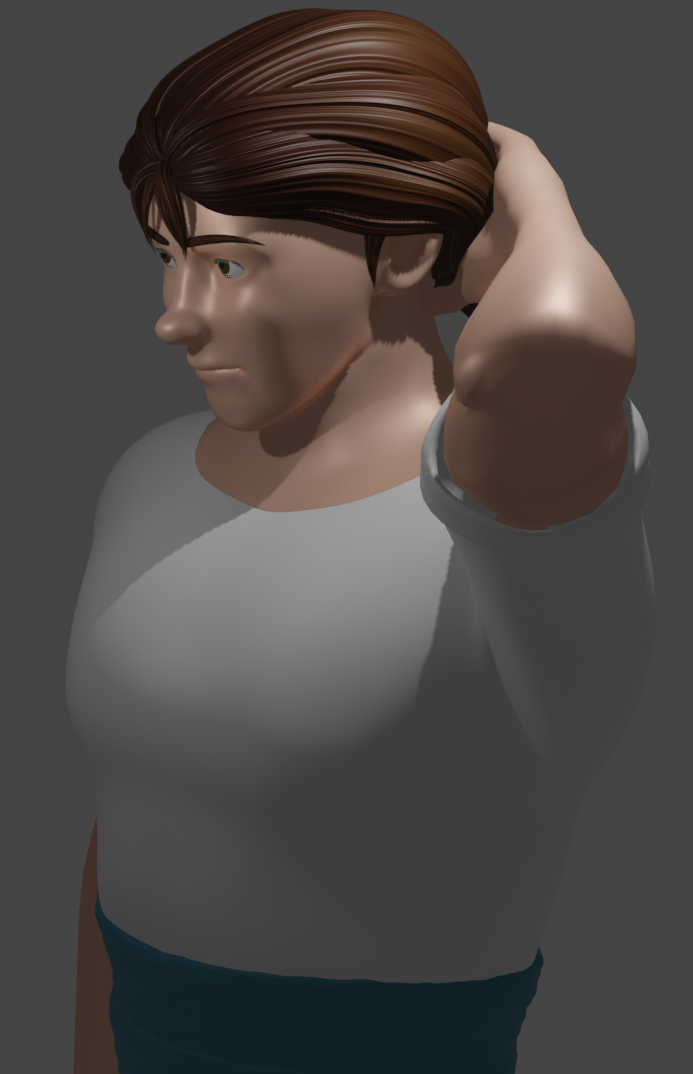
\includegraphics[width=\textwidth]{figures/ragazzo.png}
          \caption{Ragazzo}
      \end{figure}

    \column{0.33\textwidth}
      \begin{figure}
          \centering
          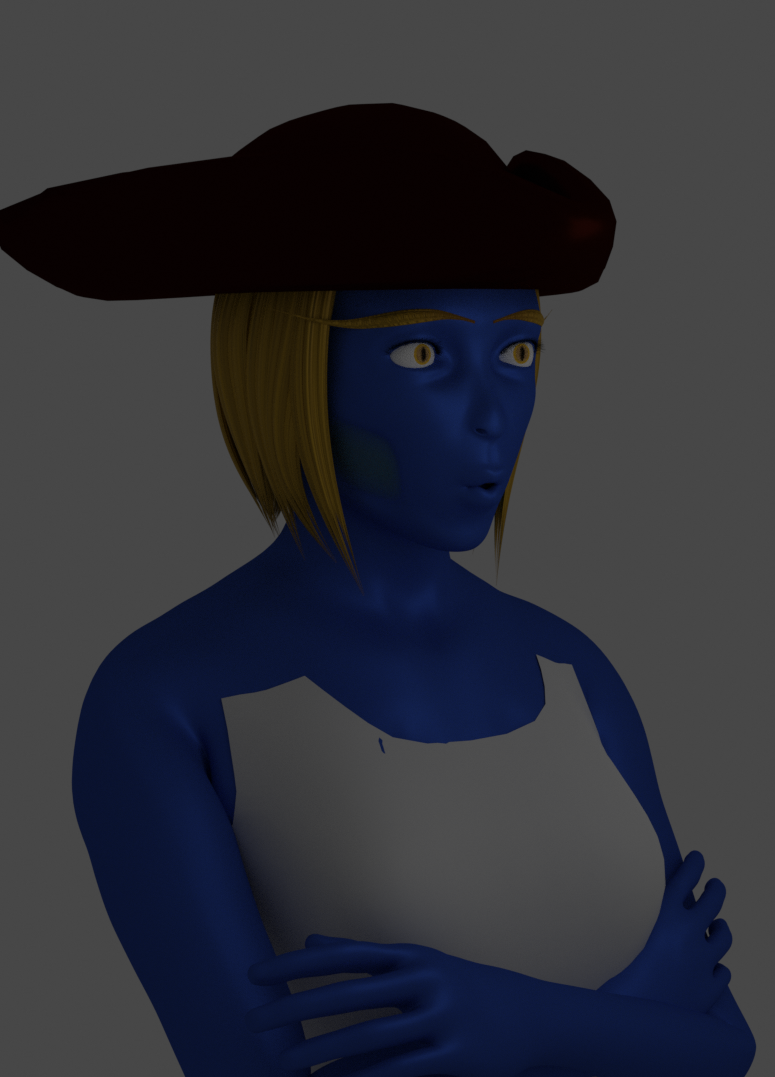
\includegraphics[width=\textwidth]{figures/Capitana.png}
          \caption{Capitana}
      \end{figure}
  \end{columns}
\end{frame}

\section{Concetti di animazione}

\begin{frame}{Rappresentazioni di rotazione}
  \begin{columns}[T,onlytextwidth]
    \column{0.33\textwidth}
    Euler
      \begin{itemize}[<+- | alert@+>]
        \item Concettualmente semplice
        \item Complessa e confusa in pratica
        \item L'ordine delle rotazioni è importante
        \item Gimbal lock e interpolazioni spezzate
      \end{itemize}

    \column{0.33\textwidth}
      Quaternions
      \begin{itemize}[<+- | alert@+>]
        \item No gimbal lock
        \item Interpolazione diretta e dolce
        \item Semplifica i calcoli
        \item Interpolazioni consistenti e predicibili
      \end{itemize}
      
    \column{0.33\textwidth}
    Matrici
      \begin{itemize}[<+- | alert@+>]
        \item Qualsiasi tipo di trasformazione
        \item Parenting
        \item Constraints
        \item Armature deform
      \end{itemize}
  \end{columns}
\end{frame}

\begin{frame}{FK (Forward Kinematics)}
  \begin{itemize}[<+- | alert@+>]
    \item Figure complesse come quella umana
    \item Approccio naive
		\item Precisione del posizionamento
    \item Difficile animare azioni comuni
  \end{itemize}
\end{frame}

\begin{frame}{IK (Inverse Kinematics)}
  \begin{itemize}[<+- | alert@+>]
    \item Figure complesse come quella umana
    \item Approccio inverso
		\item Semplifica le animazioni
    \item Complessa da calcolare
  \end{itemize}
\end{frame}


\begin{frame}[fragile]{IK - Lo Jacobiano}
  \begin{columns}[T,onlytextwidth]
    \column{0.5\textwidth}
    $
    \begin{bmatrix}
        \dfrac{\partial p_x}{\partial \theta_1} & \dfrac{\partial p_x}{\partial \theta_2} & \dots & \dfrac{\partial p_x}{\partial \theta_n} \\[2ex]
        \dfrac{\partial p_y}{\partial \theta_1} & \dfrac{\partial p_y}{\partial \theta_2} & \dots & \dfrac{\partial p_y}{\partial \theta_n} \\[2ex]
        \vdots & \vdots & \ddots & \vdots \\[2ex]
        \dfrac{\partial \alpha_z}{\partial \theta_1} & \dfrac{\partial \alpha_z}{\partial \theta_2} & \dots & \dfrac{\partial \alpha_z}{\partial \theta_n} 
    \end{bmatrix}
    $
    \column{0.5\textwidth}
		Matrice di derivate parziali corrispondenti alla differenza della posizione attuale dell'end-effector rispetto alla posizione obiettivo.
		\begin{alertblock}{Proprietà}
			\begin{itemize}
				\item Soluzione iterativa
				\item Simile al metodo del simplesso
			\end{itemize}
    \end{alertblock}
	\end{columns}
\end{frame}


\section{Progettazione}
\begin{frame}{Rigging} % I rig dei modelli devono essere pensati in base alle animazioni da realizzare
  \begin{table}
					\caption{Diversi tipi di rig necessari un una figura umana in base ai compiti che deve eseguire}
		\begin{tabular}{lcr}
			\toprule
			Porzione del rig & Compito & Soluzione\\
			\midrule
			Braccia & raggiungere e gesticolare & IK e FK\\
			Mani & afferrare & FK\\
			Gambe & correre e camminare & IK\\
			\bottomrule
		\end{tabular}
	\end{table}	
\end{frame}

\section{Produzione}
\begin{frame}{Animazioni}
	\metroset{block=fill}
	\begin{columns}[T,onlytextwidth]

		\column{0.45\textwidth}
		\begin{exampleblock}{IK}
		camminata\\
		corsa\\
		raggiungere
		\end{exampleblock}
		\begin{exampleblock}{FK}
		raggiungere\\
		afferrare
		\end{exampleblock}

		\column{0.45\textwidth}
		\begin{exampleblock}{Curve}
		camminata\\
		corsa\\
		inseguimento spaziale
		\end{exampleblock}
		\begin{exampleblock}{Cicli}
		camminata\\
		corsa\\
		sparatorie
		\end{exampleblock}
	\end{columns}
\end{frame}

{\setbeamercolor{palette primary}{fg=orange}
\begin{frame}[standout]

Risultato

\end{frame}
}

\end{document}
